\documentclass{article}

\usepackage[hidelinks]{hyperref}
\usepackage{graphicx}
\graphicspath{{./imgs/}}

\usepackage{listings}

\usepackage[style=authoryear]{biblatex}
\addbibresource{b38ro-report.bib}
\renewcommand*{\nameyeardelim}{\addcomma\space}
\usepackage{bm}

\usepackage{parskip}
\setlength{\parindent}{12pt}

\usepackage{amstext} % for \text macro
\usepackage{array}   % for \newcolumntype macro
\newcolumntype{L}{>{$}l<{$}} % math-mode version of "l" column type

\usepackage{float}

\renewcommand{\labelenumii}{\arabic{enumi}.\arabic{enumii}}
\renewcommand{\labelenumiii}{\arabic{enumi}.\arabic{enumii}.\arabic{enumiii}}
\renewcommand{\labelenumiv}{\arabic{enumi}.\arabic{enumii}.\arabic{enumiii}.\arabic{enumiv}}

\begin{document}

\title{B38RO - Robotics Group Project}
\author{Muhammad Abban - H00427641 \and Abdul Maajid Aga - H00431236  \and Laith Samir Mohamed - H00427630 \and Tejas Arcot - H00381441}
\date{\parbox{\linewidth}{\centering%
  School of Engineering and Physical Sciences \endgraf
  Heriot Watt University Dubai \endgraf\bigskip
  May 2024 }}
\maketitle
\bigskip

\tableofcontents
\newpage

\section{Introduction}

Nowadays, robotics has become an significant fragment of modern society. From diminishing monotonous tasks in factories to allowing surgeons to perform remote, intricate operations, robots have been advancing and unlocking possibilities that were previously unattainable through basic human labour. This is primarily due to their enhanced efficiency, precision, and accuracy, as well as their ability to achieve long-term cost savings and reduce downtime.

In this report, we utilised the robot simulation platform CoppeliaSim, known as the ”Swiss Army Knife” of robotic simulators, and used Robot Operating System (ROS2) to develop and test algorithms implementing the theory behind robot control, enabling our robotic manipulator to play tic-tac-toe against a human.

\section{Theory}

\subsection{Orientation}

Rotation Matrices are redundant. They give us a redundant description of the frame orientations. Rotation Matrices contain 9 elements and 6 constraints, which implies that 3 parameters are more than sufficient to describe the orientation of a body. Thus, we sought a minimal representation of orientation with 3 independent parameters.

This minimal representation can be obtained by using three angles, which are known as Euler angles. Several conventions of Euler angles (24, to be exact) exist, depending on the axes being rotated and the order of their rotation.

Conventional algorithms for kinematics however use mostly quaternions to represent orientation, with 4 independent parameters. To perform conversion to “ZYX” Euler angles, we have used the Bernardes and Viollet method, because the classical methods of converting a quaternion to Euler angles are complicated, relying on multiple matrix multiplications, whereas this method is 30 times faster than mentioned classical method \autocite{bernardesQuaternionEulerAngles2022}.

\subsection{Kinematics}

Forward kinematics is the computation of the end effectors’ cartesian position and orientation using the joint variables and links. By solving forward kinematic equations, one can determine the exact coordinates and orientation of the end effector in cartesian space. To solve forward kinematics, the three common methods are trigonometry (Geometric method), Denavit-Hartenberg convention, and screw theory (Product of exponentials formula) \autocite{stevensForwardKinematics}.

Inverse kinematics on the other hand deals with the reverse problem, it is the computation of the joint configuration required to achieve a desired end effector position and orientation. There are two distinct methods for solving the inverse kinematics, one is to analytically solve the equation and the other is to solve it iteratively, which means that a simplified version of the equation is calculated and evaluated repeatedly over time. Common numerical methods are Newton-Raphson method, gradient descent, cyclic coordinate descent and particle swarm optimization.

The Jacobian is a matrix which relates the robot joint velocities to its end-effector velocities through a linear transformation parameterized by the joint states. The Jacobian matrix is indispensable for understanding and controlling robotic motion, providing a vital link between joint space and Cartesian space. Its applications extend across various aspects of robotics, including velocity and force analysis, singularity detection, and solving inverse kinematics problems \autocite{craigIntroductionRoboticsMechanics2014}.

\subsection{Denavit-Hartenberg convention}

Our robot arm, the ‘Kinova Gen3-Lite’ is a 6 DOF robot, and its DH parameter table is as follows \autocite{KINOVAGen3Lite2021}:

\begin{center}
\begin{tabular}{| L | L | L | L | L |}
\hline
\bm{i} & \bm{a_{i}} & \bm{\alpha_{i}} & \bm{d_{i}} & \bm{\theta_{i}} \\ \hline
1 & 0 & \pi/2 & 128.3+115 & q_{1} \\
2 & 280 & \pi & 30 & q_{2}+\pi/2 \\
3 & 0 & \pi/2 & 20 & q_3+\pi/2 \\
4 & 0 & \pi/2 & 140+105 & q_4+\pi/2 \\
5 & 0 & \pi/2 & 28.5+28.5 & q_{5}+\pi \\
6 & 0 & 0 & 105+130 & q_{6}+\pi/2 \\ \hline
\end{tabular}
\end{center}

\section{Software}

\subsection{Framework}

Our software stack utilises Robot Operating System (ROS) \autocite{doi:10.1126/scirobotics.abm6074} as a communications library for our various programs to work in parallel and share data. The method of interacting between the arm was through joint angles and velocities, which are published on a JointTrajectory topic. Our application involved moving the arm to specific cartesian positions and orientations, as well as monitoring the state state of the joint’s positions and velocities. To handle the maths behind both the inverse and forward kinematics, as well as calculating velocity Jacobians of the arm, we utilised functions provided in the python library named "PyKin" \autocite{jinPykin2024}, which internally uses the Unified Robotics Description Format (URDF) of the arm modelled as a chain of links to solve kinematics problems. 

All of the code, simulation files, and other documentation for this project are open-sourced under an MIT license \footnote{\url{https://github.com/Abban-Fahim/b38ro-project}}.

\begin{figure}[h]
    \centering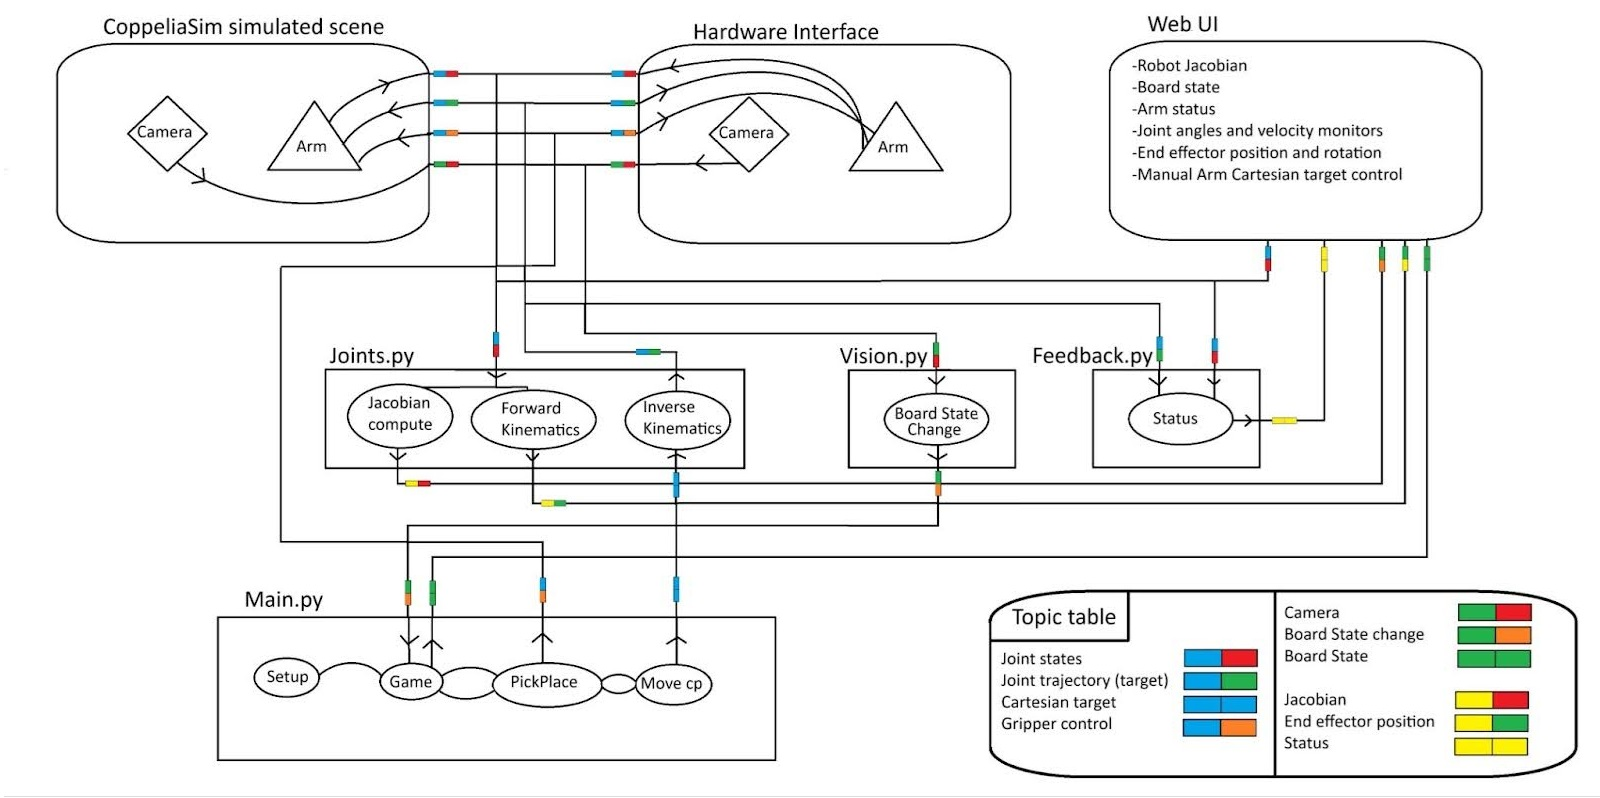
\includegraphics[width=0.85\textwidth]{diagram}
    \caption{High level overview of the ROS nodes}
\end{figure}

We also developed a Graphical User Interface (GUI) using web technologies to allow visual monitoring of joint angle and velocities, end-effector cartesian position and orientation, and the arm’s real-time Jacobian, as well as have inputs to manually control the arm to cartesian positions. The GUI's real-time graphs also helped in verifying our implementation of the "Status" variable, as the forward kinematics could be compared to the individudal joint angles at any given time.

\begin{figure}[h]
    \centering
    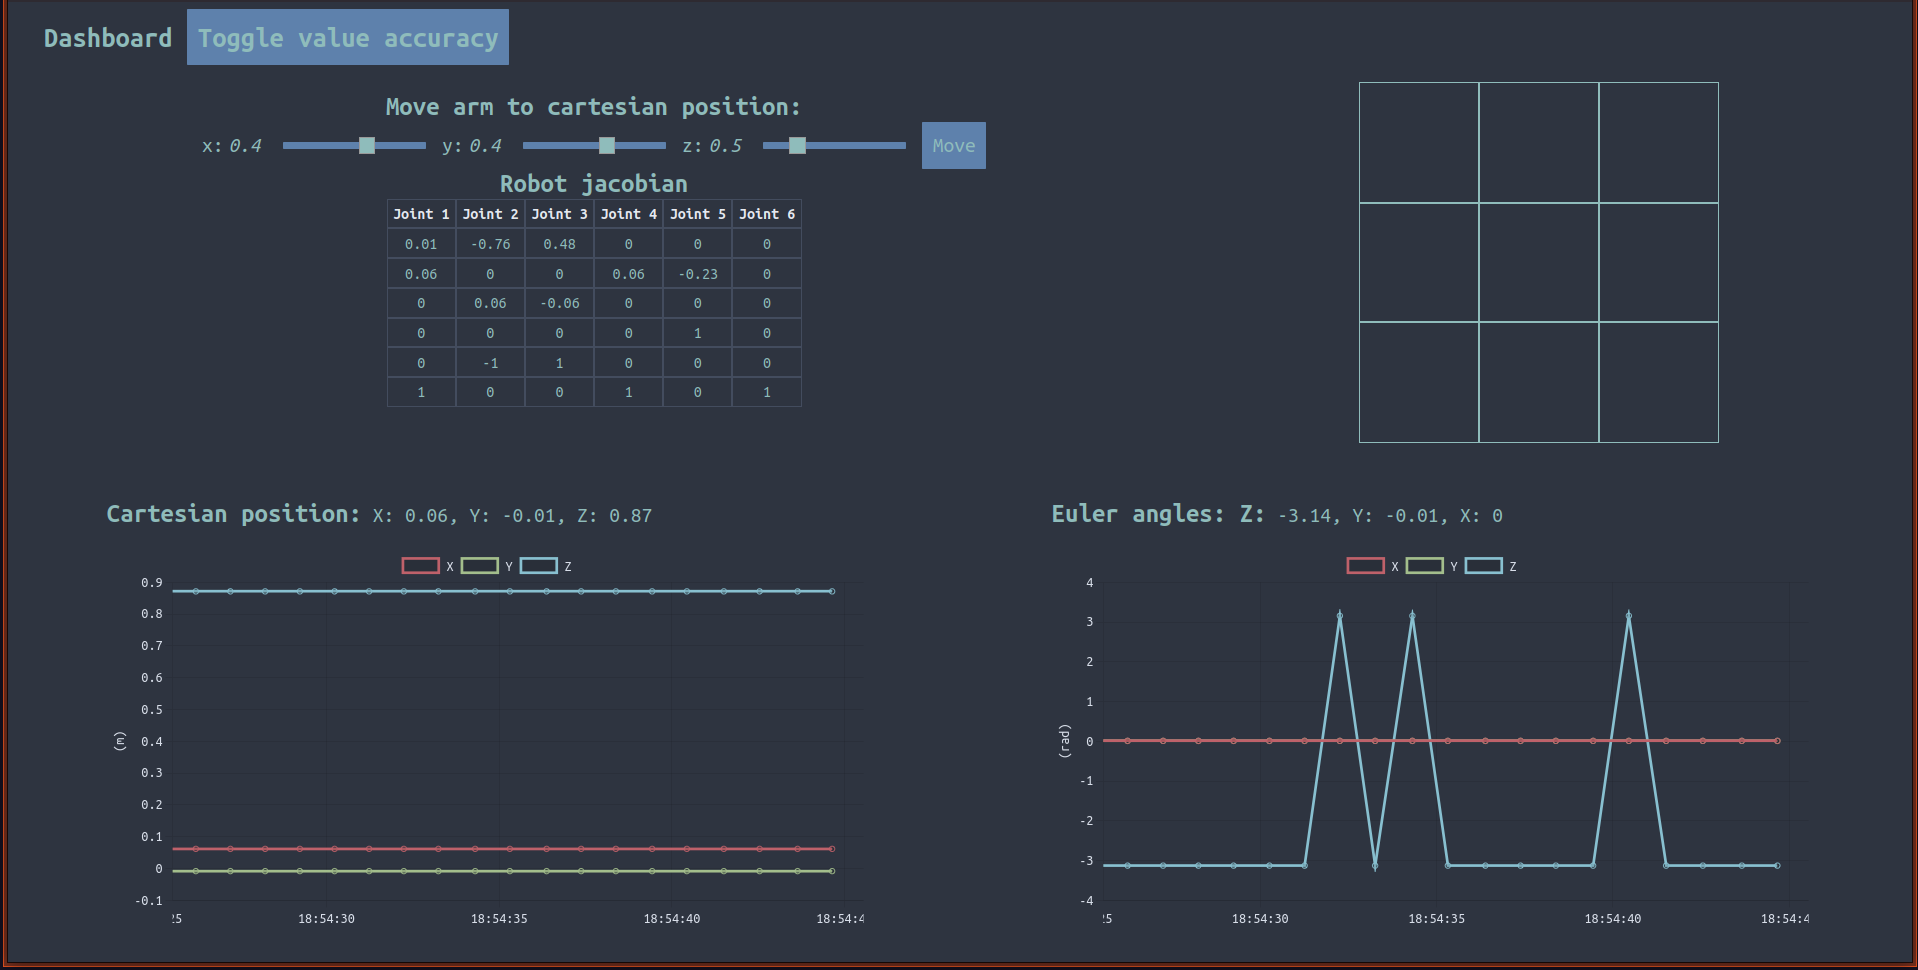
\includegraphics[width=0.45\textwidth]{website1}
    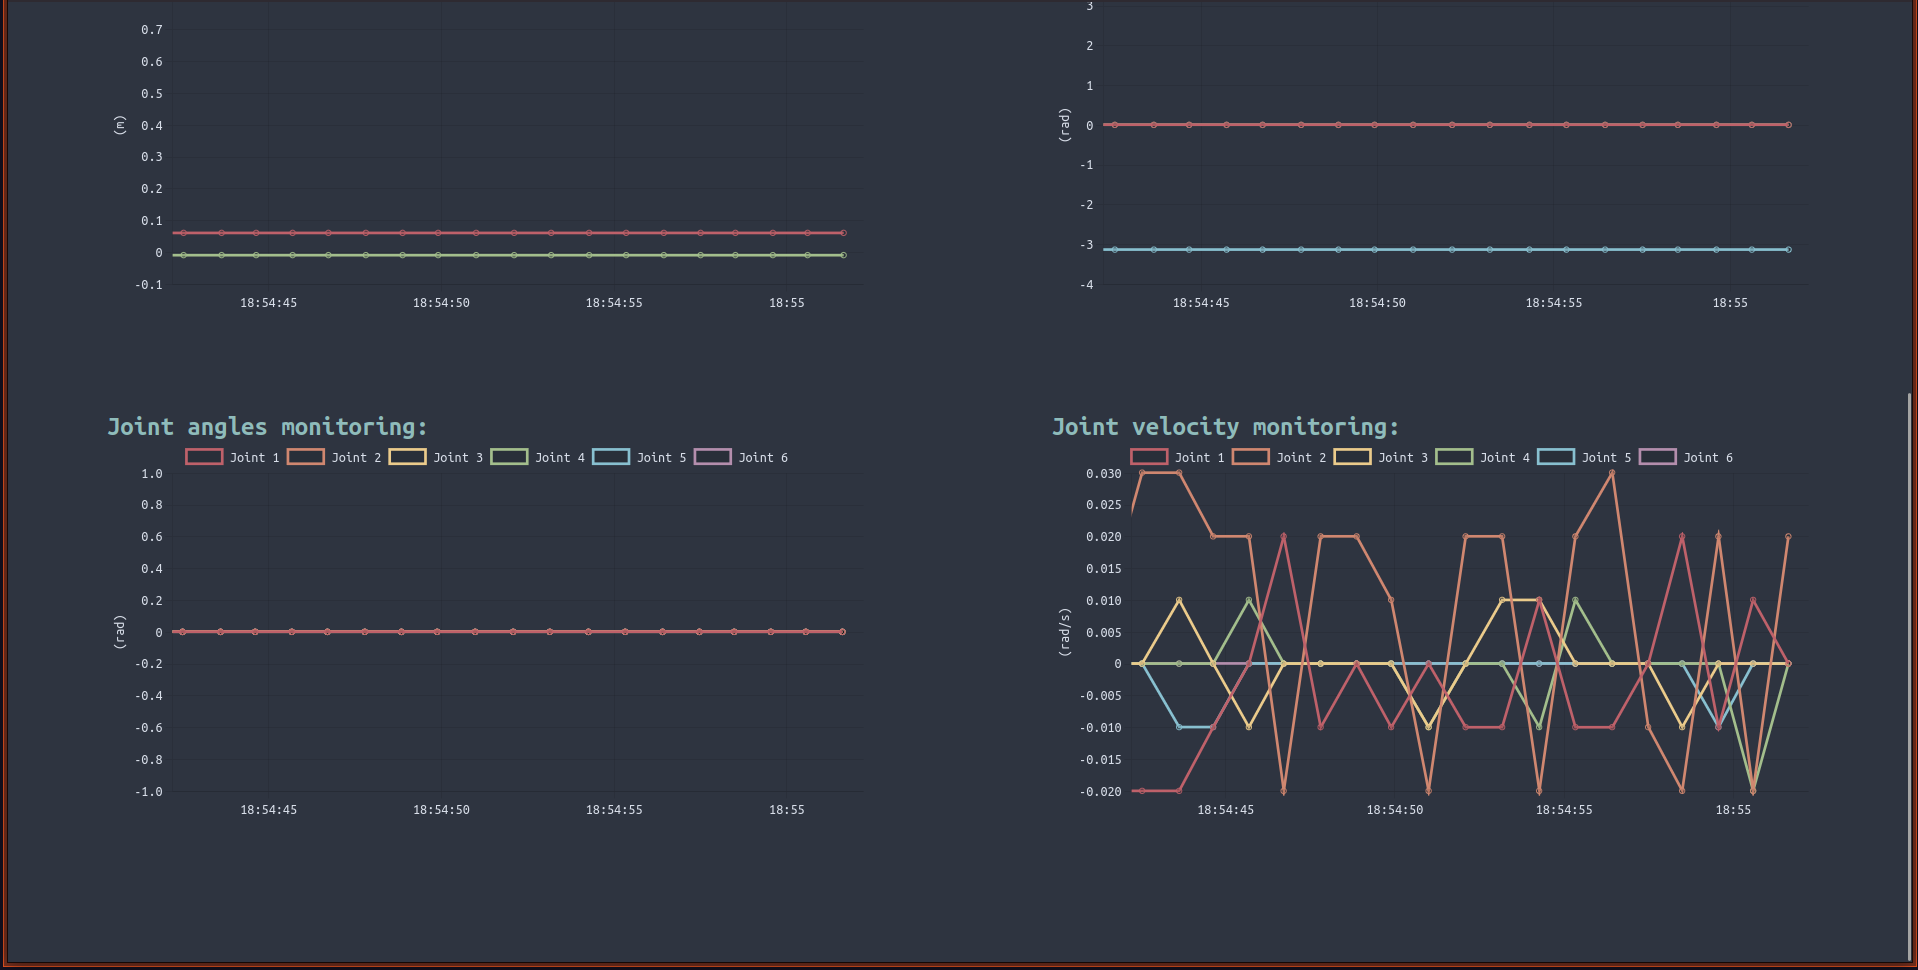
\includegraphics[width=0.45\textwidth]{website2}
    \caption{Our GUI}
\end{figure}


\subsection{Simulation}

\begin{figure}[H]
    \centering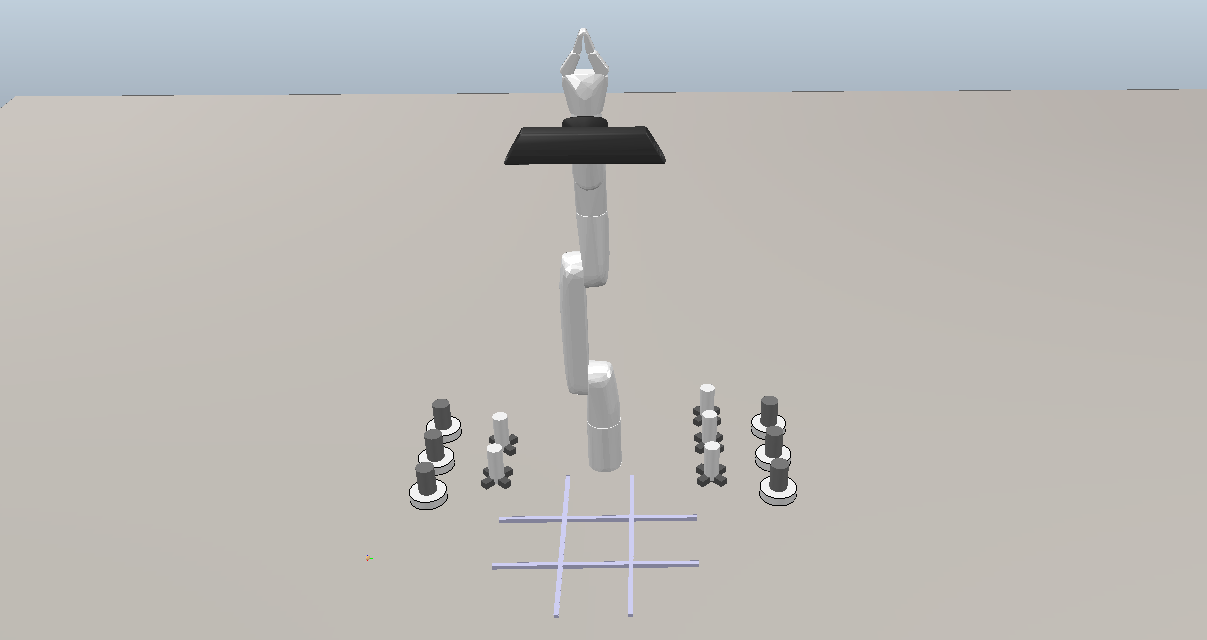
\includegraphics[width=0.75\textwidth]{scene}
    \caption{Our simulation scene}
\end{figure}

Our choice of simulation environment was “CoppeliaSim” \autocite{rohmerCoppeliaSimFormerlyVREP2013}, formerly known as “V-Rep”, due to its cross-platform availability, easy-to-use user interface, and availability of many objects and sensor components. Our choice of robotic manipulator was the Kortex Gen3 Lite from KinovaRobotics, due to its flexibility of having 6 degrees of freedom (6-DOF) and a gripper as an end-effector. Its small size also made it ideal for a scenario of human-robot interaction 

Since the arm was not available as one of the stock robot manipulators, we had to manually import the arm using the official 3d models and URDF files from the manufacturer’s repository \autocite{KinovaroboticsRos_kortex2024}, while encountering some trouble during this process due to outdated documentation.

We controlled the robot’s operation using internal scripts and the ROS2 plugin. By utilising the joint and motion planning modules, we were able to reliably move the robot to any set of valid joint angles and velocities without self-collision. To ensure the imported Kinova Gen3 Lite simulation worked like the real robot, we subscribed the robot to the “joint\_trajectory” topic, which the hardware interface exposes to receive target angles, velocities and acceleration for low-level control.

For the gripper, we used the "gripper\_pose" topic to send open/close commands. The hardware interface advertised an action server which we sent commands to. In simulation, we imported the gripper’s URDF and attached it at the end-effector link. Due to the nature of CoppeliaSim’s physics, we used the documented method of gripper behaviour, which is done using a dummy joint at the gripper and a force sensor to detect if an object is between the gripper. When an object is detected inside the gripper during closing it links the object to the dummy point, and unlinks when opening, creating the illusion that the object is being picked up/dropped.


\subsection{Game logic}

For the simulation scene, we created a simple fixed tic-tac-toe grid with pieces modelled as shapes attached to a stick that the arm can grip. For our main game logic, we have a Finite State Machine (FSM) like framework that has the following states: 

\begin{figure}[h]
    \centering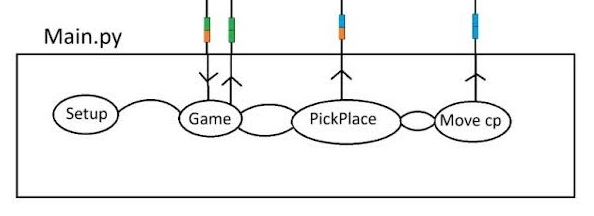
\includegraphics[width=0.75\textwidth]{game}
    \caption{FSM-like diagram of control flow}
\end{figure}

\begin{enumerate}

    \item Setup
        \begin{enumerate}
            \item Contains the initializations needed for ROS2 and some of our own functions to calculate the cartesian positions of the game board for the robot to drop at and to pick up from. Also decides on whether the arm or player goes first and records the player's move if they move first.
            \item The functions we made to calculate cartesian positions grid points works in a highly scalable way by generating all of the board’s line equations and working out the midpoints of intersections and then the midpoints of the squares. We have it setup to generate said line equations and points when given the cartesian positions of any two opposing corners of the board and returns a 9 field array with all given cartesian positions to drop at. Future work is to extend our use of Hough transformations and line detection to gain said equations.
        \end{enumerate}
    \item Game
        \begin{enumerate}
            \item Decides what the next action for the arm is and sends it to the pickplace function 
            \item Decision is done by a minimax tree algorithm. It works by generating a tree of all possible moves and results and determining what each endgame generated results in, for each given leaf (end) the AI wins it gains 10 points, tie gives 0 and losses give -10 points. The leaf values are added up and attributed to their given branch moves, the branch with the highest value is the one that has the best move.
        \end{enumerate}
    \item Pick and Place
        \begin{enumerate}
            
            \item The pickplace algorithm gets the move to do, position of next nought piece to pick up and the cartesian positions array, and decides the set of moves the arm will take to pick up the piece, move the piece and drop it above the wanted position.
                
                \begin{enumerate}
                    
                    \item The pickplace does the move in 3 parts : 

                    \item First, move to above the part we want to pickup, then move down slowly (while keeping straight down orientation ) to where the part is inside the grippers, then close grippers, then move up slowly (while keeping straight down orientation)

                    \item Second, move above the middle of the board (above by a distance of 50cm), then move above dropping point, then move down slowly (keeping straight down orientation), then open grippers when part is just above ground, then move up slowly (keeping straight down orientation)

                    \item Third, the robot moves to the neutral position, which we decided to be straight up as it provides the benefit of the real arm recalibrating automatically when in this state.  

                \end{enumerate}
                    
            \item The pickplace algorithm calls the Move to Cartesian positions function with coordinates for each arm movement 
        
        \end{enumerate}

    \item Move to Cartesian positions 

        \begin{enumerate}

            \item Move to cartesian position when called generates and sends the cartesian target ros2 message, which gets received by the IK controller, which calculates and sends the target angles to the robot arm. Then it waits a fixed amount of time to alow the arm to move. Future work is to replace the time wait with a status dependent  wait. 
            \item Move to cartesian position split is the same as Move to cartesian position, but splits the move into multiple moves to points equally spread out between the current position of the arm and target position. We use this for moving down above pieces or to dropping pieces. Because due to the nature of the normal path planning any moves, downwards/upwards directly, does not keep the orientation of the end effector whilst moving. Giving a high chance that the arm knocks down pieces whilst moving to them.Splitting the move into multiple smaller moves removes the problem as the change in orientation becomes insignificant and subdues the risk of part knockdown. 
        
        \end{enumerate}
\end{enumerate}

\subsection{Testing on hardware}

The major challenge presented by executing trajectories on the actual hardware were singularities. These are joint configurations where arm movement becomes restricted due to lining up of two joint axes causing the arm to lose a degree of freedom. Mathematically, the determinant of the velocity jacobian becomes undefined and we can no longer calculate for Inverse Kinematics from these points. These points are found primarily at the boundaries of the arm’s reachable workspace, and in certain loci within the workspace \cite{craigIntroductionRoboticsMechanics2014}. 

When the arm enters such a configuration, an on-board fault controller throws an exception and stops the arm from moving. The challenge then lies in monitoring this fault controller, resetting it, and bringing the arm back into a non-fault position, such as the all zero angle configuration, which we achieved through a bash script.

\subsection{Vision, feedback and further improvements}

We implemented a simple vision system to track changes to the state of the board. In order to simplify the vision logic, we gave the nought and cross pieces distinctive colours and positioned the camera directly above the grid. The image processing pipeline involved:

\begin{enumerate}
    \item converting the image to one-channel grayscale
    \item using erosion with a 6x6 kernel to reduce the width of the grid lines
    \item using Canny edge detection to extract the sharp boundaries in the image
    \item using Hough Transformation in polar-coordinates to extract only the lines that make up the grid
    \item using polar parameters of the lines to section the grid into nine individual squares
    \item tallying the colours of all pixels in these sections to find out which piece is inside, or lack thereof
\end{enumerate}

\begin{figure}[h]
    \centering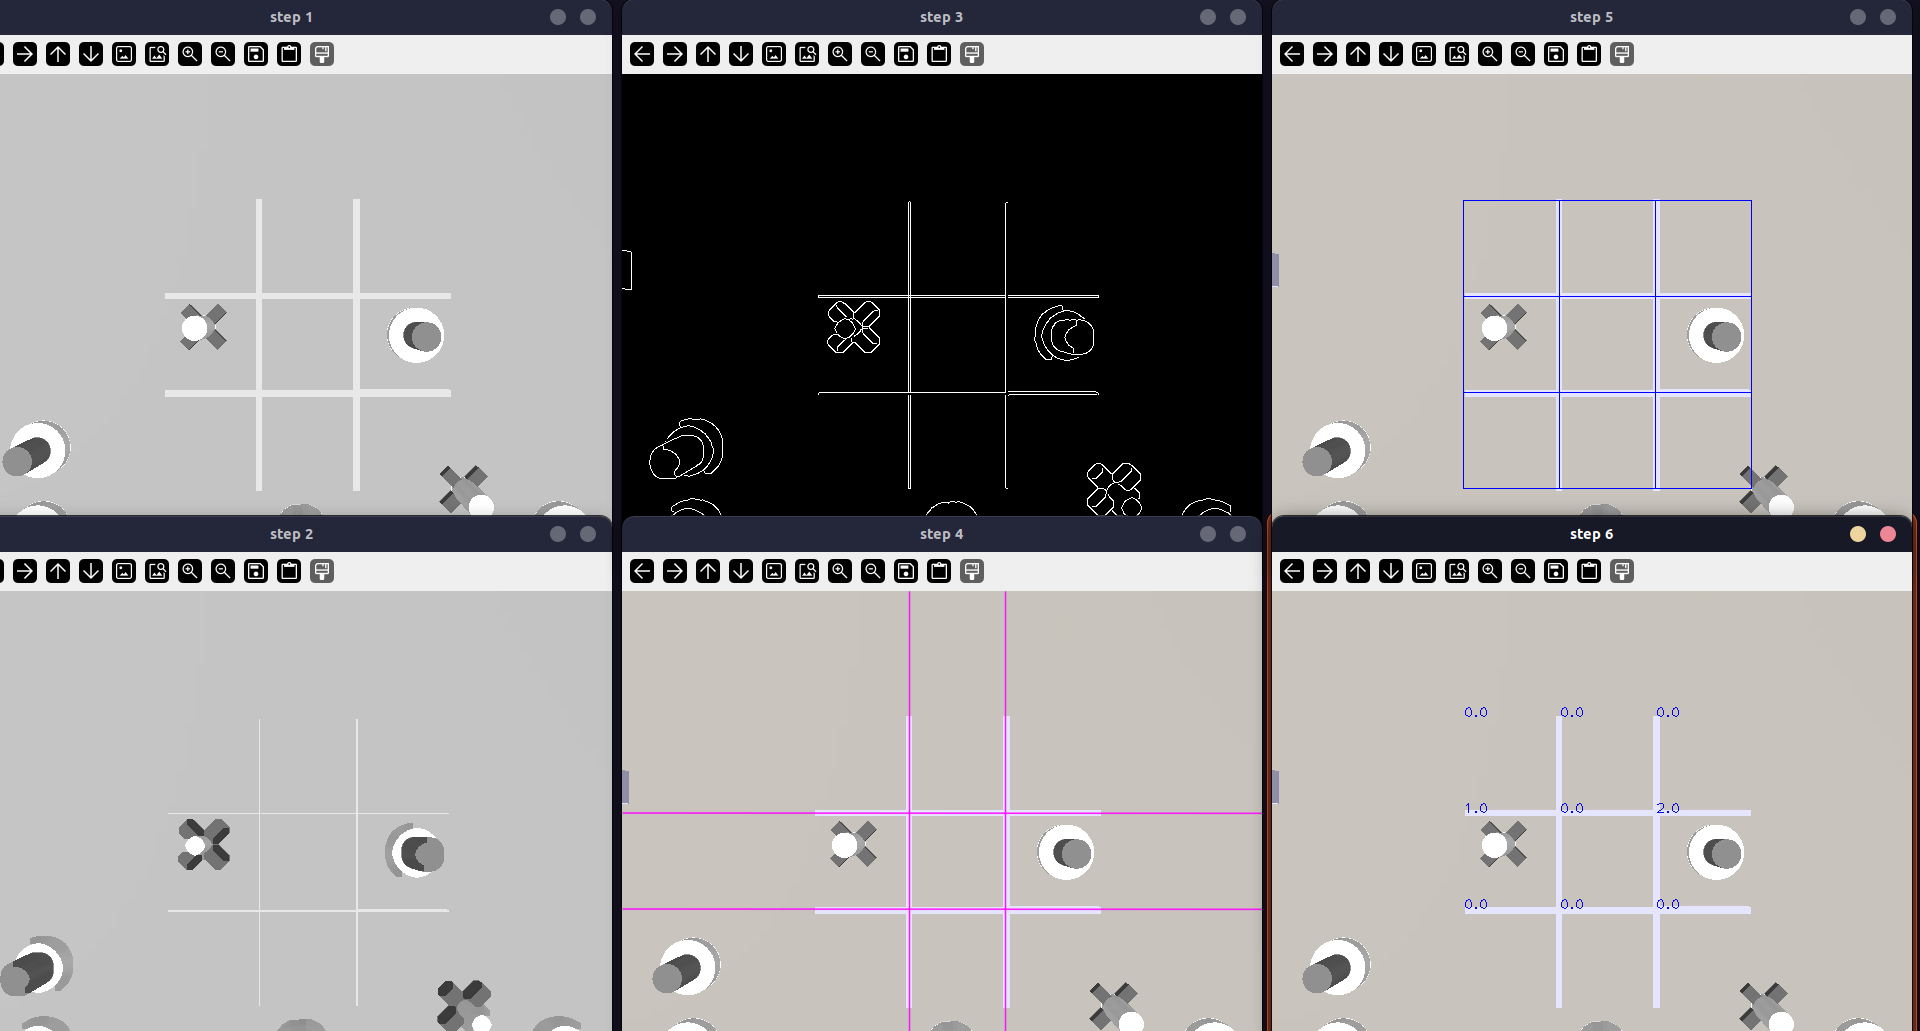
\includegraphics[width=0.85\textwidth]{vision}
    \caption{The computer vision pipeline visualised (1 = cross, 2 = nought)}
\end{figure}

We also introduced a feedback topic, "Status," which monitors and compares the joint states with the target joint trajectories. This topic indicates whether the robot is actively moving towards the target angles or is in an idle state. Although the code and simulation are functional, we are actively working on improving and optimising the entire pick-and-place framework to behave more like a FSM, and hence enhance consistency and performance.

Some of the improvements we are working on: 

\begin{itemize}
    \item To utilise our robot status topic in the pick and place to enable the arm to automatically proceed to the next step, rather than relying on a fixed wait time between each step. The primary challenge in implementing this feature arises from Python's single-threaded nature and the operation of ROS2. This combination means that any non-fixed loops dependent on the robot's status can cause the entire program, including ROS2 communication, to pause, leading to infinite pauses. The  main workaround is to rely on multithreading libraries, by having the game thread pause when the robot is not idle and unpause when the robot reaches its target and sets its status to idle.
    \item To use the fault controller to automatically detect and rectify hardware interface exceptions regarding invalid configurations, or to find a way to overwrite or modify the onboard computer to ignore such errors.
    \item To use the camera to track the game pieces, game board, and arm relative to each other, we could potentially utilise ArUco markers. This approach would enable the framework to function without being restricted by scene setup difficulties. 
\end{itemize}

\section{Tasks}
The coursework has 8 aims and targets:

\begin{enumerate}
    \item bring the end effector to any desired Cartesian position,
    \item make the manipulator move with any desired end-point translational and rotational Cartesian velocity,
    \item make the robot follow any given Cartesian position trajectory,
    \item read, write and plot the joint angles of the robot in any configuration,
    \item read or compute and then write and plot the Cartesian positions and Euler-angles of the end-point of the robot manipulator,
    \item read or compute and then write the Jacobian matrix of the manipulator,
    \item plot the joint angles, Cartesian position, and Euler angles of the end-point effector
    \item be able to move the robot with keyboard buttons and/or external remote or wired controllers (e.g. game joysticks).
\end{enumerate}
  
Most of the aims and targets are done by the UI and main game task: targets 1,4,5,6 and 7.
For targets 3 and 8 we made a controller node, which reads the current position from the end effector position topic and publishes an offset Cartesian target depending on the controller status. 

\begin{figure}[h]
    \centering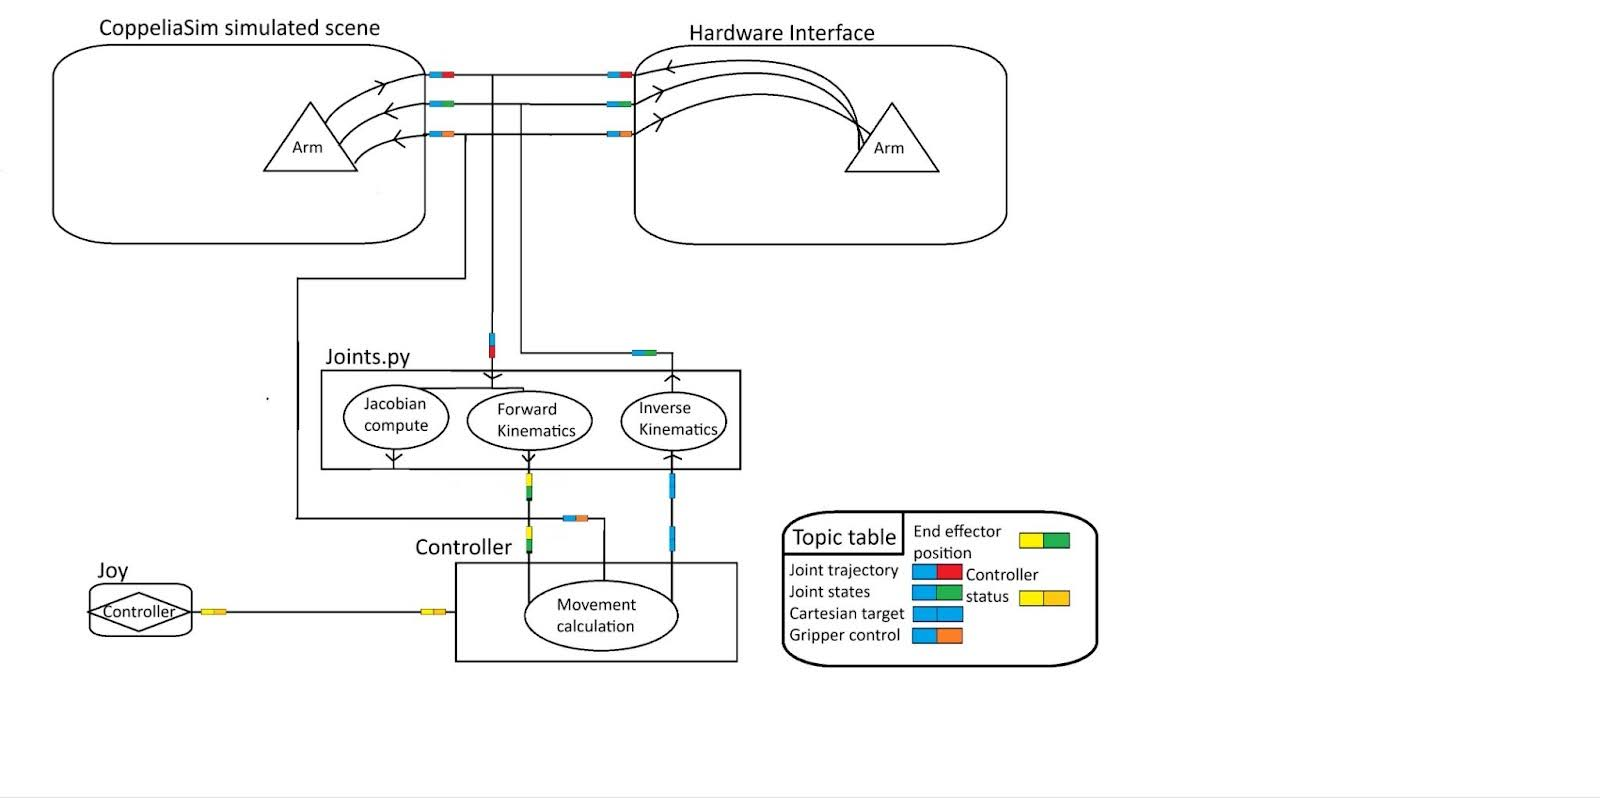
\includegraphics[width=0.75\textwidth]{controller}
    \caption{ROS nodes for the using the controller}
\end{figure}

 For target 2 we made a modified version of Joints.py, which uses the inverse of the Jacobian and a modified Joint trajectory topic containing 6 extra variables (one for each joint) dictating the velocity of each joint, which inturn makes us able to control the endpoint translational and rotational velocity. By recalculating and publishing at fixed movement intervals we are able to control the rotational and translational velocity to varying accuracies (dependent on refresh rate).

\section{Conclusion}

In conclusion, our project has shown effective integration and control of a robotic manipulator within the CopeliaSim simulator, by leveraging ROS2 and external custom libraries. In addition to that we have supplemented our work with a perception system to demonstrate the robots ability to interact with changes in its live environment based on real-time visual feedback. Despite us overcoming most challenges, we encountered a few that were beyond our skill-set and require extensive research to solve, for example Python's single threaded execution making us unable to detect and wait for when the arm finishes a trajectory, and using vision for board state detection outside of the simulated scene. 

Our application is based on Pick-and-Place mechanisms that have wide-ranging uses in various sectors to improve accuracy and efficiency of processes like manufacturing and soldering. Combining these with computer vision and workspace calibration, there are various applications of our simulations in industrial and research environments. With further research, the potential of our work can go well beyond a game of tic-tac-toe. Our experience can be adapted and used for innovation in the robotics field, paving the way for advancements in automated systems that can be tailored to a variety of complex tasks in real-world scenarios.

\printbibliography[heading=bibintoc]

\end{document}
